\subsection{Предварительная обработка текстов}
\subsubsection{Общие сведения}

\par
Часто решение задачи, каким-либо образом связанной с моделированием естественного языка, требует предварительной обработки текста, содержащей в себе:
\begin{itemize}
    \item приведение текста к единому регистру (обычно, нижнему);
    \item токенизацию -- разбиение текстов на более мелкие единицы (токены), которые могут быть различными по размеру, в зависимости от задачи;
    \item морфологическую разметку: с целью различать омонимы, несущие отличные семантические роли;
    \item удаление стоп-слов (слов, носящих излишне частотный или разреженный характер);
    \item лемматизацию (приведение слова к лемме -- нормальной <<словарной>> форме) или стемминг (сокращение слова до его основы);
    \item векторизацию слова: представление токенов в качестве численных векторов для последующей обработки.
\end{itemize}

\bigskip\par
Так как выбранный язык исследования английский, то морфологическая разметка особого результативного прироста не даст и ее можно опустить. После приведения текста к единому регистру и токенизации необходимо составить словарь слов текстов. Для оптимального построения словаря выполняется редуцирование слов (лемматизация) и удаление излишне частых и разреженных слов. Рассмотрим эти процессы подробнее.  
\subsubsection{Лемматизация и удаление стоп-слов}
\par
Минимальную информацию о текстовых данных можно получить с помощью понятий частоты. Закон Ципфа гласит, что наиболее часто употребимых слов лишь небольшое количество, тогда как подавляющее большинство слов используются существенно реже: частота любого слова в корпусе текстов обратна пропорциональна его рангу в таблице частот слов этого текста. Рассмотрим один из датасетов, на которых будет происходить последующее обучение моделей: отзывы на фильмы с платформы IMDB. Построим закон Ципфа в логарифмических координатах рис. \ref{fig:zipf}:
\[\ln r + \dfrac{1}{\alpha}\ln \omega_r = f(r),\]
где $r$ -- ранг слова в таблице частот, $\alpha \approx 1$ -- константа, $\omega_r$ -- абсолютная частота слова.
\begin{figure}[H]
    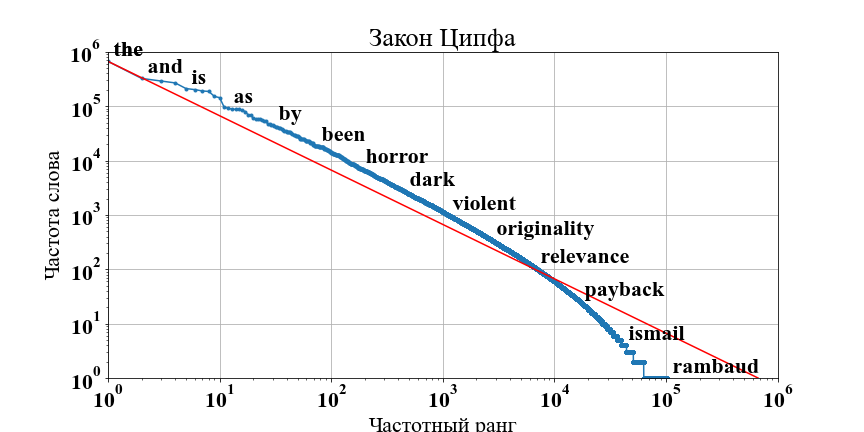
\includegraphics[scale=0.5]{zipf.png}
    \caption{Закон Ципфа на датасете IMDB}
    \label{fig:zipf}
\end{figure}

\bigskip\par
Явно заметен тренд к линейности, однако даже есть явное отклонение в районе слов с высоким ранжированием. Рассмотрим на распределения частот для позитивных и отрицательных комментариев (рис. \ref{fig:distribution_tokens_before_lemmatization}):
\begin{figure}[H]
    \centering
    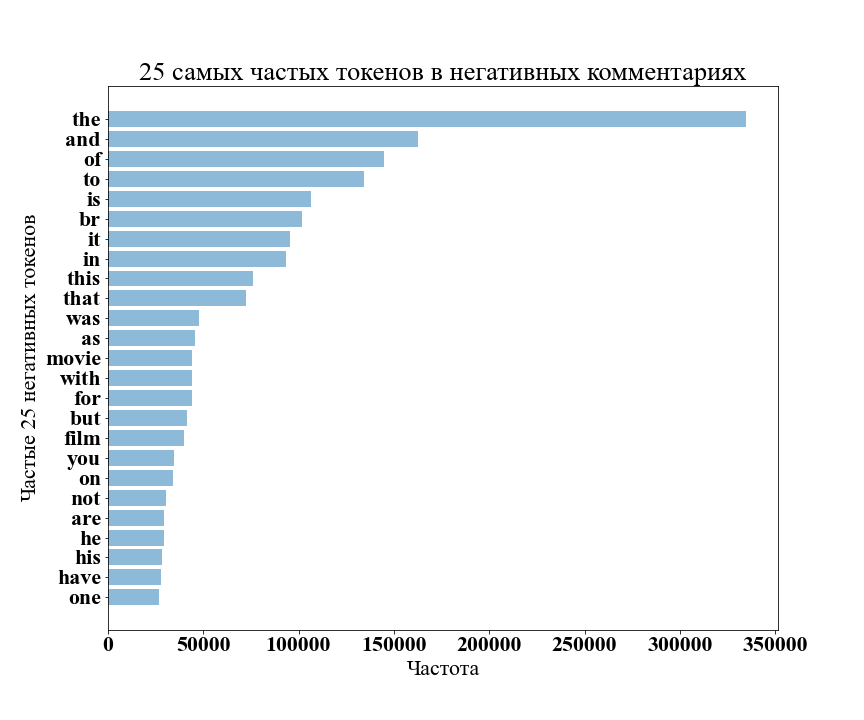
\includegraphics[scale=0.5]{negative.png}
    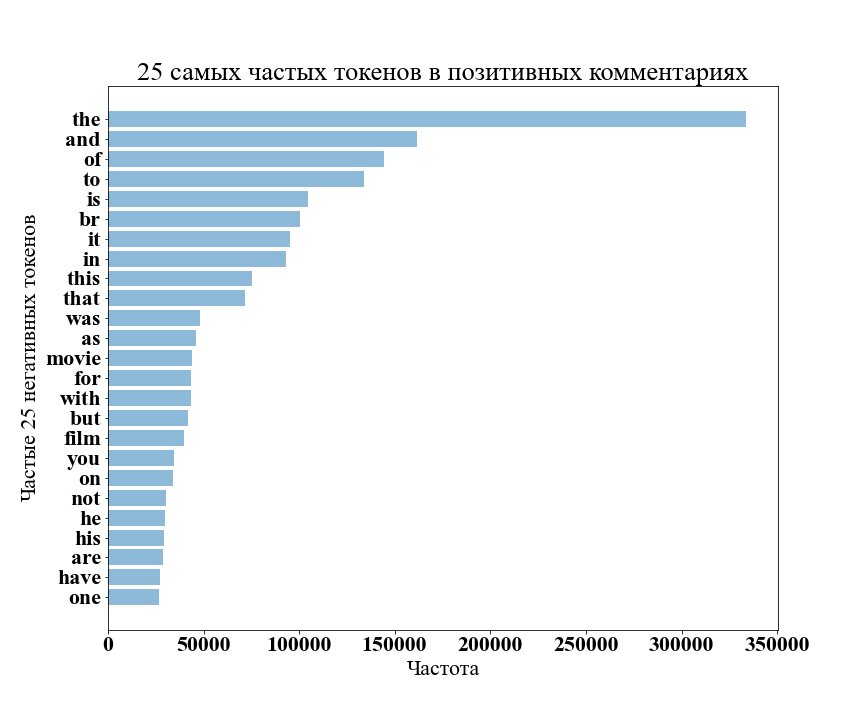
\includegraphics[scale=0.5]{positive.png}
    \caption{Самые частые слова в позитивных и негативных комментариях}
    \label{fig:distribution_tokens_before_lemmatization}
\end{figure}

\bigskip\par
Слова настолько часто встречающиеся усложняют процесс поиска закономерностей в текстовых данных. Похожее влияние оказывают и излишне редко встречающиеся слова: зачастую это либо профессионализмы или диалектизмы, либо слова с ошибками. Поэтому, помимо оптимальности построения словаря, в рамках задачи решение о применении этих методов предобработки текстов приведет к упрощению поиска заномерностей в итак сложно структурированных данных. Рассмотрим частотные характеристи после лемматизации и удаления стоп-слов (рис. \ref{fig:distribution_tokens_after_lemmatization})
\begin{figure}[H]
    \centering
    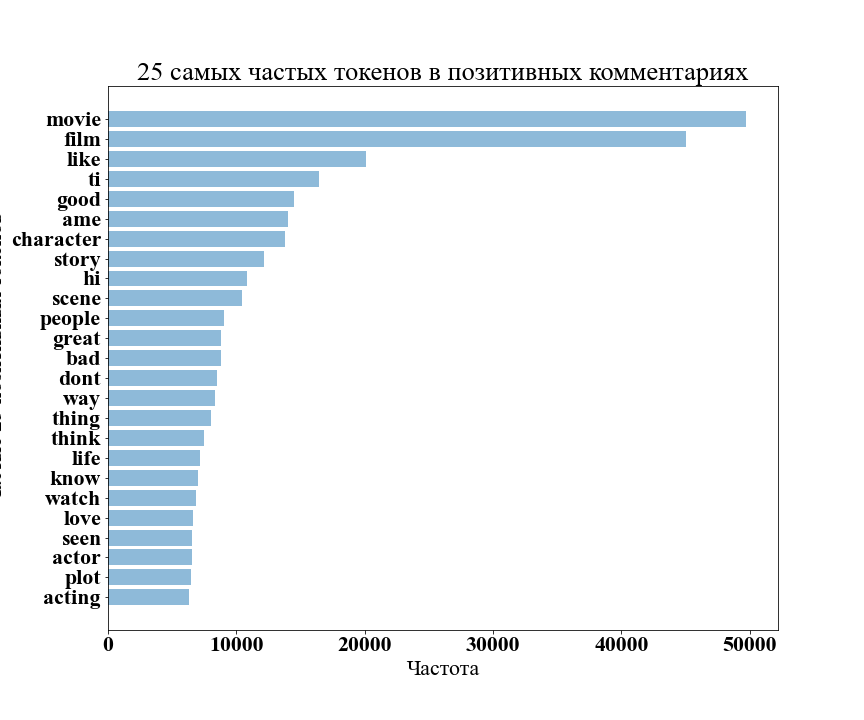
\includegraphics[scale=0.5]{positive_ac.png}
    \caption{Самые частые слова в позитивных комментариях после лемматизации и удаления стоп-слов}
    \label{fig:distribution_tokens_after_lemmatization}
\end{figure}

\bigskip\par
Позитивное влияние в виде упрощения структуры данных очевидно. Теперь необходимо представить предобработанные комментарии в векторном виде, чтобы в дальнейшем подавать их в модели глубокого обучения.

\subsubsection{Векторизация слов}
\paragraph{Bag of Words}
\par
Наиболее простым способом представления токенов в векторной форме является One Hot Encoding (OHE). Этот метод заключается в сопоставлении каждому токену вектора с размерностью, равной мощности словаря, и имеющего на всех позициях значения 0, кроме той, которая соответствует позиции самого токена в словаре, элемент с этим индексом равен 1 (рис. \ref{fig:ohe}).
\begin{figure}[H]
    \centering
    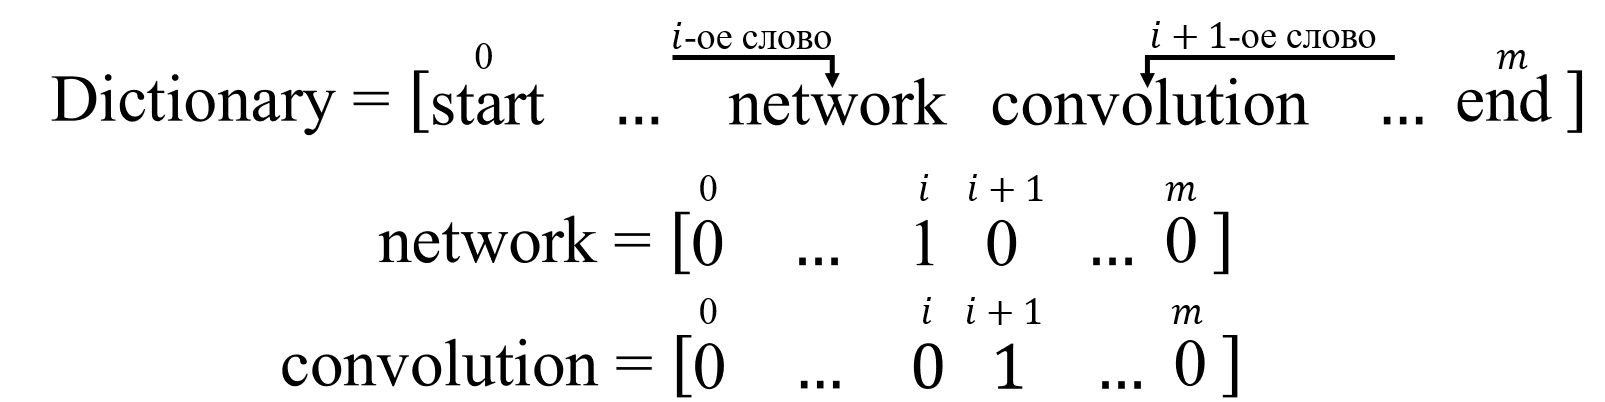
\includegraphics[scale=0.5]{ohe.png}
    \caption{One hot encoding (OHE) представление слов}
    \label{fig:ohe}
\end{figure}
\bigskip\par
Такой подход обладает достаточно закономерными недостатками:
\begin{itemize}
    \item вектора неинформативны: все векторы полученного пространства ортогональны друг другу, что не является полезным, причем большей информации о таком пространстве получить невозможно;
    \item большая размерность полученного пространства: с полученными векторами сложно оперировать функционально валидно из-за <<проклятия размерности>> \cite{curse};
    \item отсутствие возможности задать метрику в пространстве: слабая репрезентативность и отсутствие желаемых свойств пространству (арифметические операции над словами)
\end{itemize}
\bigskip\par
С целью получить количественную характеристику (частотную меру слов) применяется метод <<мешок слов>> \cite{harris54}. В работе метода выдвигается гипотеза о том, что порядок слов не несет в себе никакой информации. Получим векторы текстов путём сложения one-hot векторов токенов, в него непосредственно входящих рис. \ref{fig:bow}. 
\begin{figure}
    \centering
    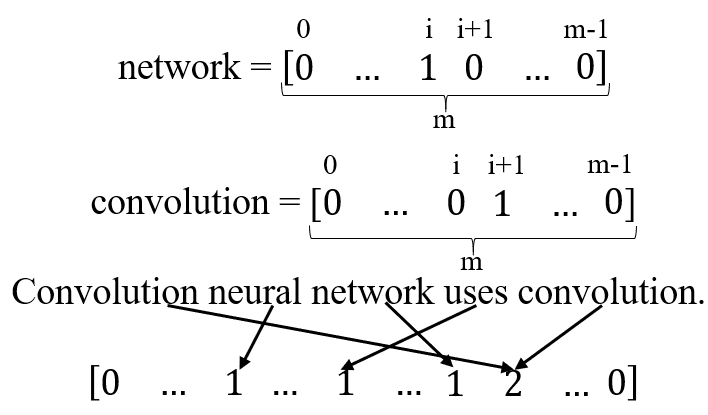
\includegraphics[scale=0.75]{bow.png}
    \caption{Bag of Words текстовое представление}
    \label{fig:bow}
\end{figure}
Такое представление так же содержит в себе немалое количество недостатков, среди которых: отсутствие информации о семантике и порядке слов. Однако эвристики и связанные с ними гипотезы оказываются полезными в дальнейшем. 
\paragraph{TF-IDF}
\par
Один из наиболее популярных способов векторизации в моделях машинного обучения. Все тексты представляются в виде матрицы $T = \left(t\right)_{d,w} = TF-IDF(w,d,D),$ где $d \in D$ -- текст, $w \in W$ -- слово в тексте. TF-IDF -- статистическая мера для оценки важности слова в контексте документа.
\[TF-IDF(w,d,D) = TF(w,d) \times IDF(w, D),\]
где $TF$ -- частота слова, которая оценивает слова в пределах документа (текста) по формуле:
\[TF(w,d) = \dfrac{n_i}{\sum\limits_{k}n_k},\]
где $n_i$ -- количество вхождений i-го слова в тексте. $\sum\limits_{k}n_k$ -- общее число слов в тексте. IDF вычисляется по формуле:
\[IDF(w,D) = \log \dfrac{|D|}{\{d_i \in D | w \in d_i\}},\]
где $|D|$ длина корпуса текстов, $\{d_i \in D | w \in d_i\}$ -- число текстов, в которых есть слово $w_i.$ 
\paragraph{Word2Vec}
\par
Word2Vec представляет собой полносвязную нейронную сеть с двумя различными архитектурами. В обоих случаях по тексту проходят скользящим окном размера $K$. Среди $K$ слов выделяют $K-1$ слов контекста и центральное слово. Первый тип Word2Vec Skip-gram (рис. \ref{fig:skipgram}) заключается в предсказывании контекста для слова:
\begin{figure}[H]
    \centering
    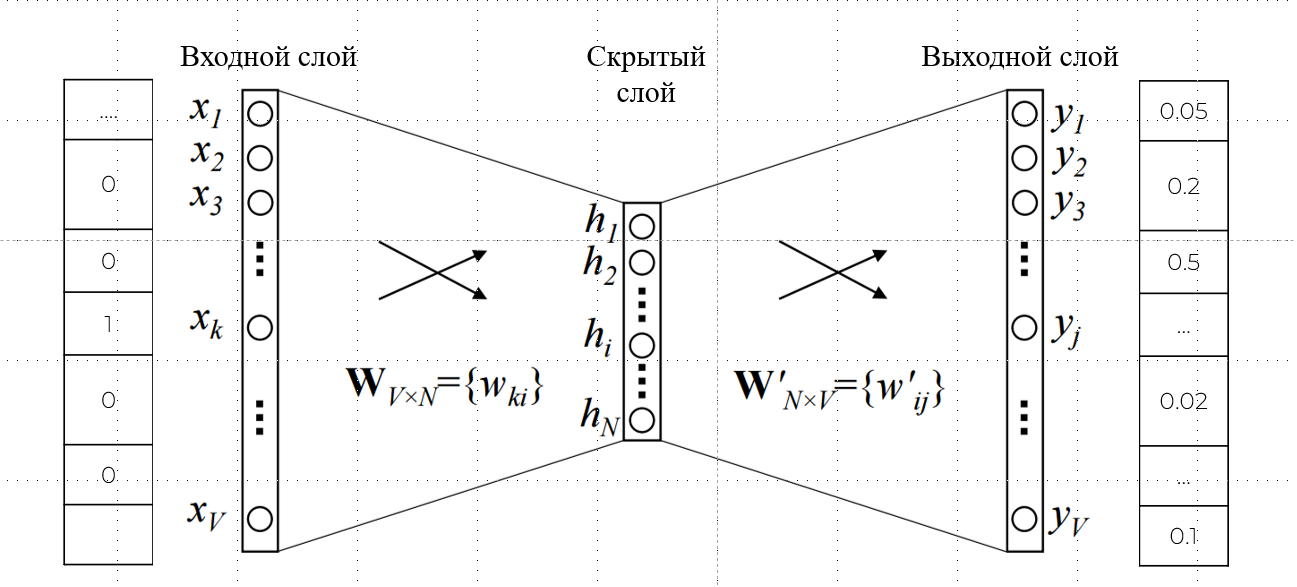
\includegraphics[scale=0.5]{skip-gram.png}
    \caption{Модель Word2Vec SkipGram \cite{mikolov2013distributed}}
    \label{fig:skipgram}
\end{figure}
\par
На выходе имеем $K-1$ мультиномиальных распределений вида:
\[P(c_k|i) = \dfrac{e^{u_{kc_k}}}{\sum\limits_{j'=1}^V e^{u_{j'}}}\]
Функция ошибки (loss Function):
\[L = -\ln P\left(c_1, \ldots, c_n| i\right) = -\sum\limits_{k=1}^{K}u_{kc_{k}} + n\ln\sum\limits_{j'=1}^V e^{u_j'}.\]
Для обучения будем максимизировать функцию правдоподобия:
\[L(\theta) = \prod_{d \in D}\left(\prod_{c \in C(i)} P(c|d; \theta)\right) = \prod_{\left(d,c\right) \in D} P(c|d; \theta),\]
где $C(i)$ -- множество возможных контекстных слов вокруг слова $i$ при обходе скользящим окном всего текста. Вектор вероятности определяется с помощью softmax вида:
\[P(c|d, \theta) = \dfrac{e^{\tilde w_c^Tw_d}}{\sum\limits{c'}e^{\tilde w_{c'}w_d}},\]
где $\tilde{w}_c$ -- вектор слова из контекста $c$, который отличается от $w_d$. Так как слова редко встречаются в контексте самих себя, то была придумана идеология использования двух разных векторов одного и того же слова (вместо одного), в первом случае слово будет выступать в качестве центрального в контексте, в другом контекстуальным. Этот метод описан в \cite{skipgram}. Выразим максимум логарифма функции правдоподобия:
\begin{gather*}
    \argmax\limits_{\theta} \prod_{(d,c)\in D} P(c|d;\theta) = \argmax\limits_{\theta} \sum\limits_{(d, c) \in D} \ln P(c|d; \theta ) =\\
    =  \argmax\limits_{\theta} \sum\limits_{(d,c)\in D} \sum\limits_{(d,c) \in D} \left(e^{\tilde{w}^T_cw_d} - \ln \sum\limits_{c'} e^{\tilde{w}_{c'}^Tw_d}\right)
\end{gather*}
\par
В статье \cite{cbow} приведен стохастический алгоритм оптимизации процедуры матричного умножения: $\sum\limits_{c} \tilde{w}_c^Tw_d$ negative sampling, заключающийся в выборе только нескольких элементов скалярного произведения весов  в качестве <<отрицательных примеров>>. Выведем измененную функцию правдоподобия:
\[\argmax\limits_{\theta} \prod_{(d,c) \in D} P((d,c) \in D; \theta) = \argmax\limits_{\theta} \]
Для простоты выразим вероятности через сигмоидную функцию активации (так как задача бинарной классификации, то softmax может быть заменен на sigmoid). Имеем:
\[P((d,c) \in D; \theta) = \dfrac{1}{1+e^{-\tilde{w}_c^Tw_d}}.\] Добавим набор отрицательных данных:
\[\argmax\limits_{\theta} \prod_{(d,c)\in D} P((d,c) \in D; \theta) \prod_{(d,c) \in D'}P((d',c') \not \in D; \theta)\]
Подставим с выражением для сигмоиды:
\begin{gather*}
    \argmax\limits_{\theta} \prod_{(d,c)\in D} P((d,c) \in D; \theta) \prod_{(d,c) \in D'} 1-P((d',c') \not \in D; \theta) = \\ 
    = \argmax\limits_{\theta} \left[\sum\limits_{(d,c)\in D} \ln P((d,c)\in D; \theta) + \sum\limits_{(d',c')\in D'} \ln(1-P((d',c')\not \in D; \theta))\right] = \\
    = \argmax\limits_{\theta} \sum\limits_{(d,c)\in D} \left[\ln \sigma(\tilde{w}_c^Tw_i) + \sum\limits_{(d,c')\in D'} \ln \sigma (-\tilde{w}_c^Tw_d)\right] 
\end{gather*}
Итоговая функция ошибки, для которой выполняется метод оптимизации:
\[L = \ln \sigma \left(\tilde{w}_c^Tw_i\right) \sum\limits_{(d,c')\in D'} \ln\sigma(-\tilde{w}_{c'}^Tw_i).\]
\bigskip\par
Модель CBOW предсказывает слово для контекста (рис. \ref{fig:cbow}):
\begin{figure}[H]
    \centering
    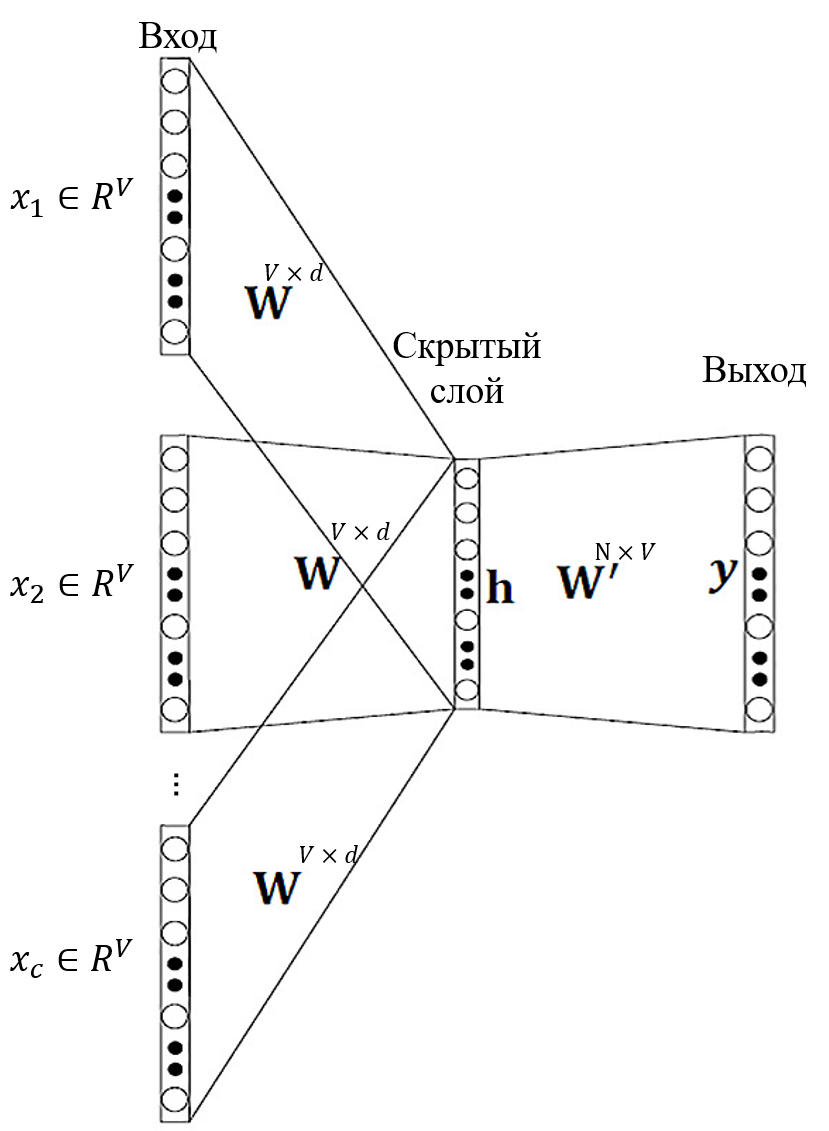
\includegraphics[scale=0.5]{cbow.png}
    \caption{Модель Word2Vec CBOW \cite{cbow}}
    \label{fig:cbow}
\end{figure}
Найдем апостериорное распределение модели с помощью softmax:
\[P(i|c_1,\ldots, c_n) = \dfrac{e^{u_j}}{\sum\limits_{j=1}^Ve^{u_j}}\]
Аппроксимируем с помощью функции потерь вида:
\[L = -\ln P(i|c_1,\ldots, c_n) = -u_j + \ln\sum\limits_{j=1}^V e^{u_j}\]
\paragraph{Embedding}
\par
С другой стороны возможно внедрение слоя Embedding непосредственно в архитектуру нейронной сети рис. \ref{fig:embedding}. Очевидным является вывод о лучшей статистике конечной модели с таким подходом, поскольку в результате обучения будет происходить подбор параметров слоя под конкретную задачу. Однако объектом исследований является значимость релевантной разницы метрики качества модели с использованием предобученных эмбеддингов Word2Vec и обучаемых слоев. Если эта разница будет незначительна, то валидным является использование предобученных моделей векторизации, поскольку они латентно содержат информацию о большем объеме слов в силу обучения на огромном корпусе текстов.
\begin{figure}[H]
    \centering
    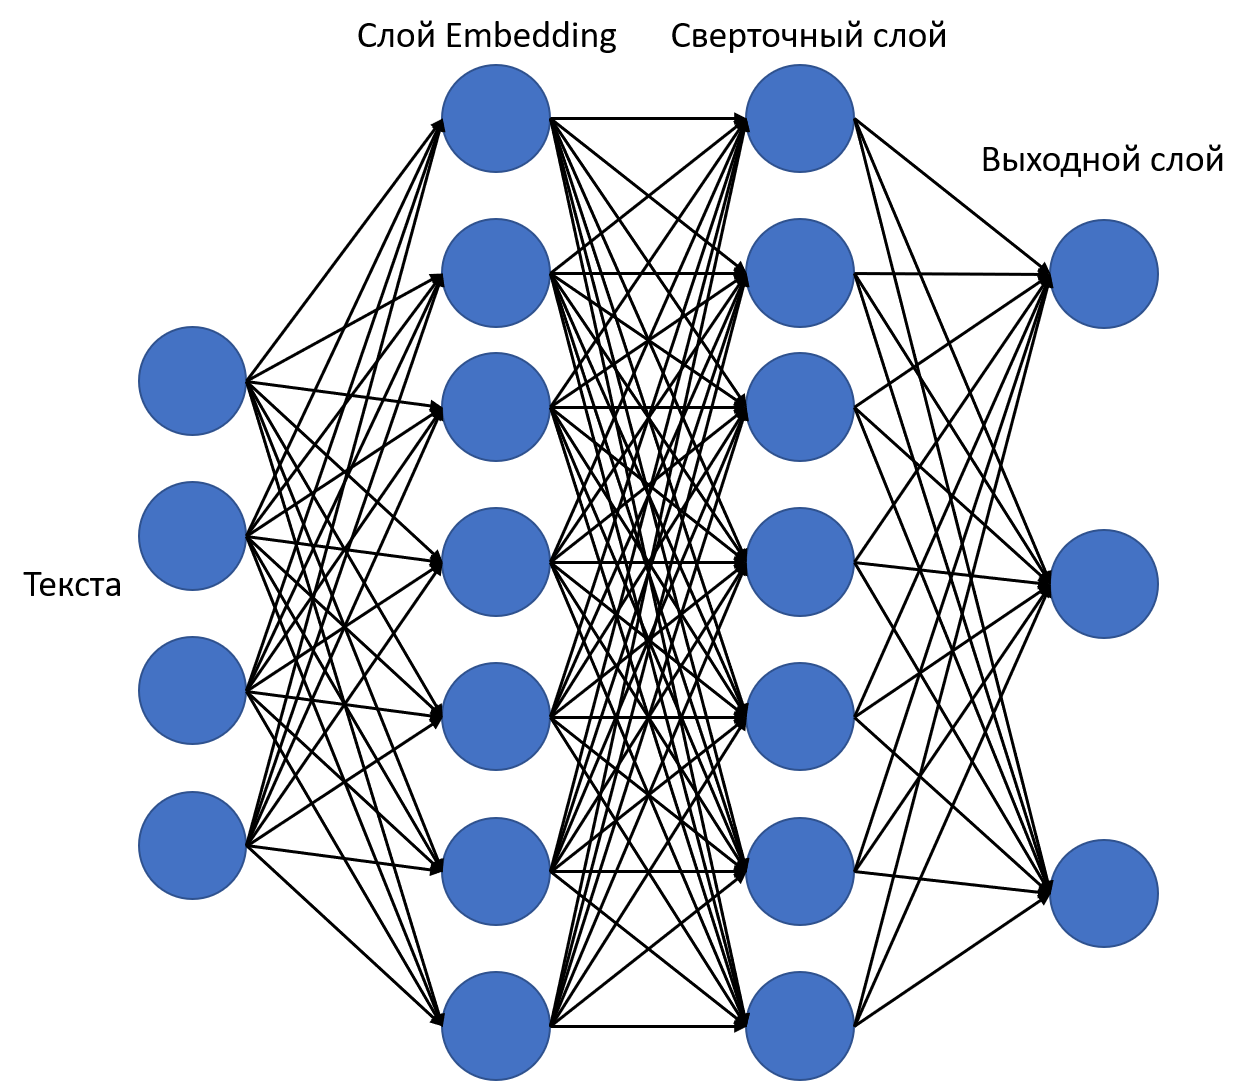
\includegraphics[scale=0.5]{embedding.png}
    \caption{Внедрение эмбеддингов непосредственно в архитектуру сети}
    \label{fig:embedding}
\end{figure}
